\subsection{Regression Analysis}
\subsubsection{Plain and Stochastic Gradient Descent}
\begin{figure}[ht!]
    \centering
    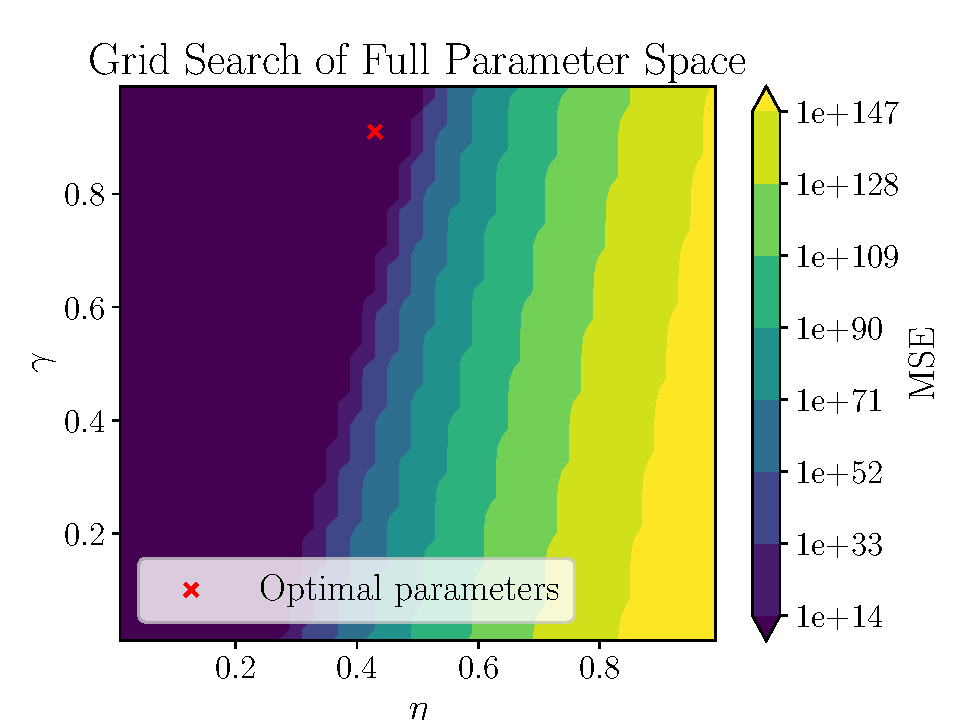
\includegraphics[width = .475\textwidth]{../figs/a_2_parameter_overview.pdf}
    \caption{Overview of the entire parameter space, plotting learning rate against momentum,  using plain gradient descent. The optimal parameters are marked with a red cross, to use as a starting point for further analysis.}
    \label{fig: param_overview}
\end{figure}
\begin{figure}[ht!]
    \centering
    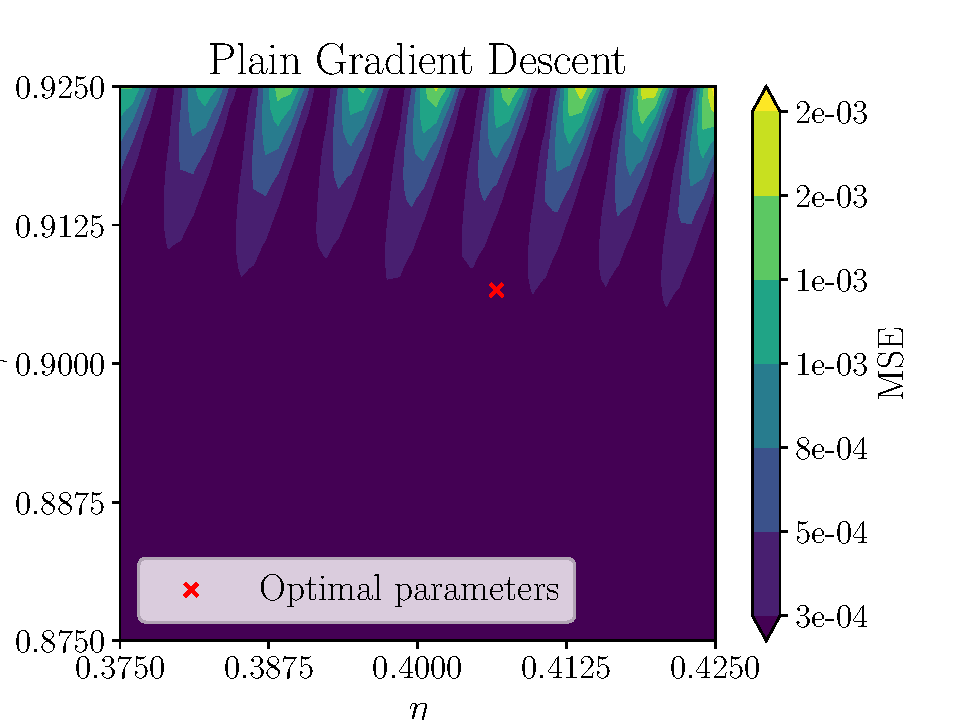
\includegraphics[width = .475\textwidth]{../figs/GD_eta_gamma.pdf}
    \caption{Narrowed down parameter space from \cref{fig: param_overview}.}
    \label{fig: param_narrowed}
\end{figure}
\begin{figure}[ht!]
    \centering
    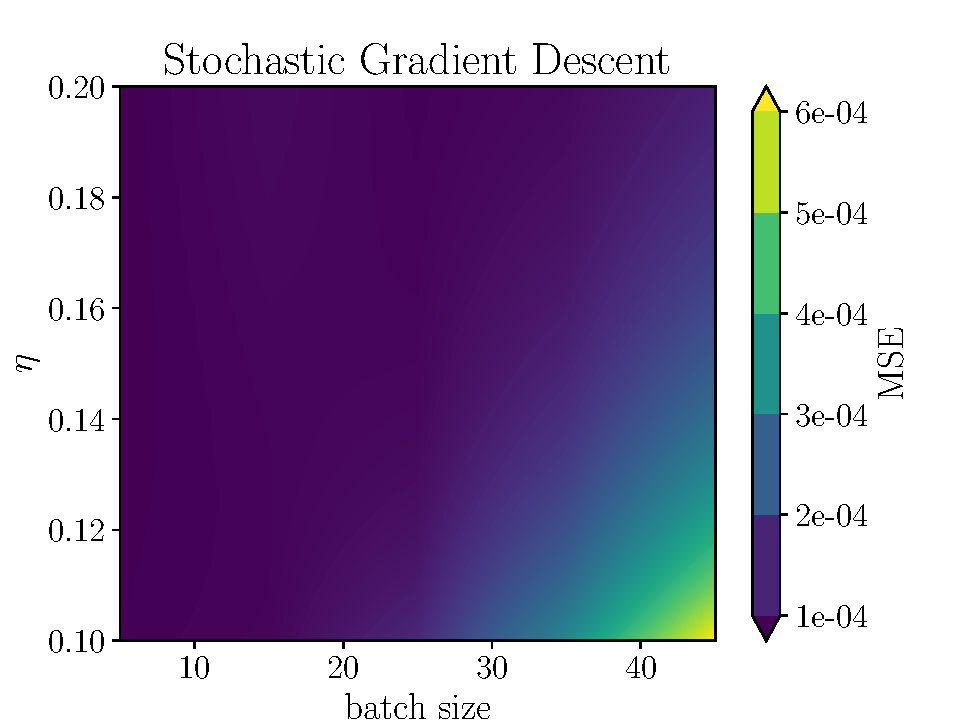
\includegraphics[width = .475\textwidth]{../figs/SGD_batch_eta_.pdf}
    \caption{Plotting batch size, against learning rate, using stochastic gradient descent.}
    \label{fig: SGD_batch_eta}
\end{figure}
\begin{figure}[ht!]
    \centering
    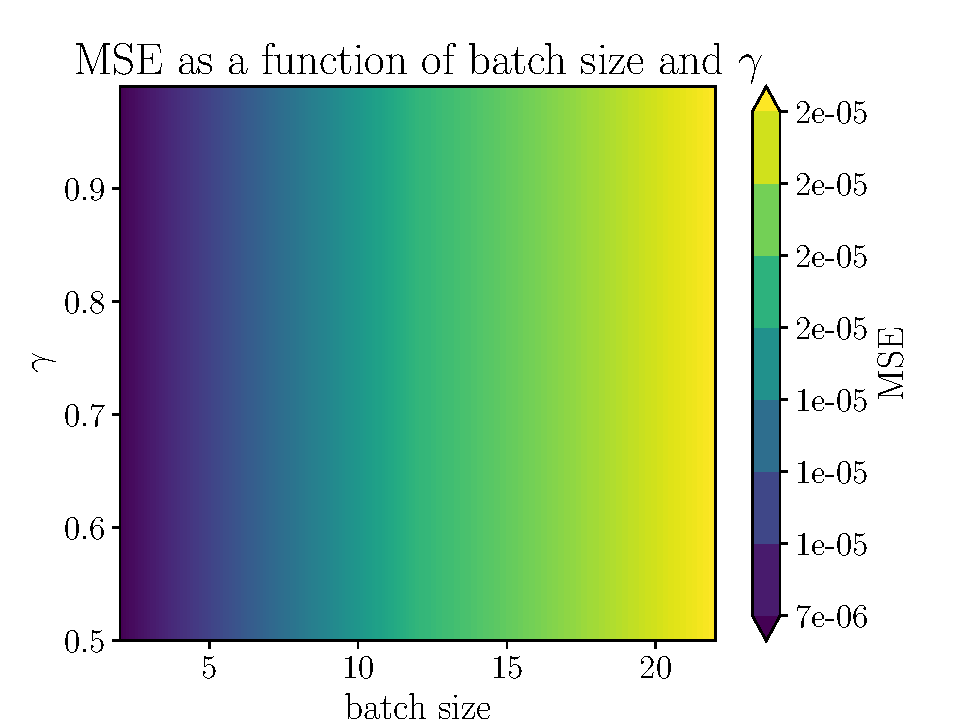
\includegraphics[width = 0.47575\textwidth]{../figs/SGD_batch_gamma.pdf}
    \caption{Plotting the batch size against the momentum, using stochastic gradient descent. Using a learning rate of $0.2$}
    \label{fig: SGD_batch_gamma}
\end{figure}

Looking at \cref{fig: param_overview} we found a region of parameters  in the upper-half , which gave the lowers MSE values. Using the best parameters found marked with a cross as a starting point, we found a good interval of values as seen in \cref{fig: param_narrowed}, with an order of magnitude around $10^{-4}$ and $10^{-3}$. In the following results, we only present the best intervals.

Continuing our search for the optimal batch number, we found between 5 and 20 batches to work well. In \cref{fig: SGD_batch_eta} without momentum. As a learning of $0.2$ gave the best results, we used this as our fixed learning rate in \cref{fig: SGD_batch_gamma} to find an optimal number of batches as a function of momentum. We see that the effect of changing the momentum is almost negligible, and that the number of batches is the most important parameter to tune. Even though we see a clear gradient in the plot, we find a large area with MSE values in the order of magnitude of \(10^{-5}\). The same is true in \cref{fig: SGD_batch_eta}, where over half of the learning rates between $0.1$ and $0.2$ give MSE values around \(10^{-4}\).

\subsubsection{AdaGrad}
\begin{figure}[ht!]
    \centering
    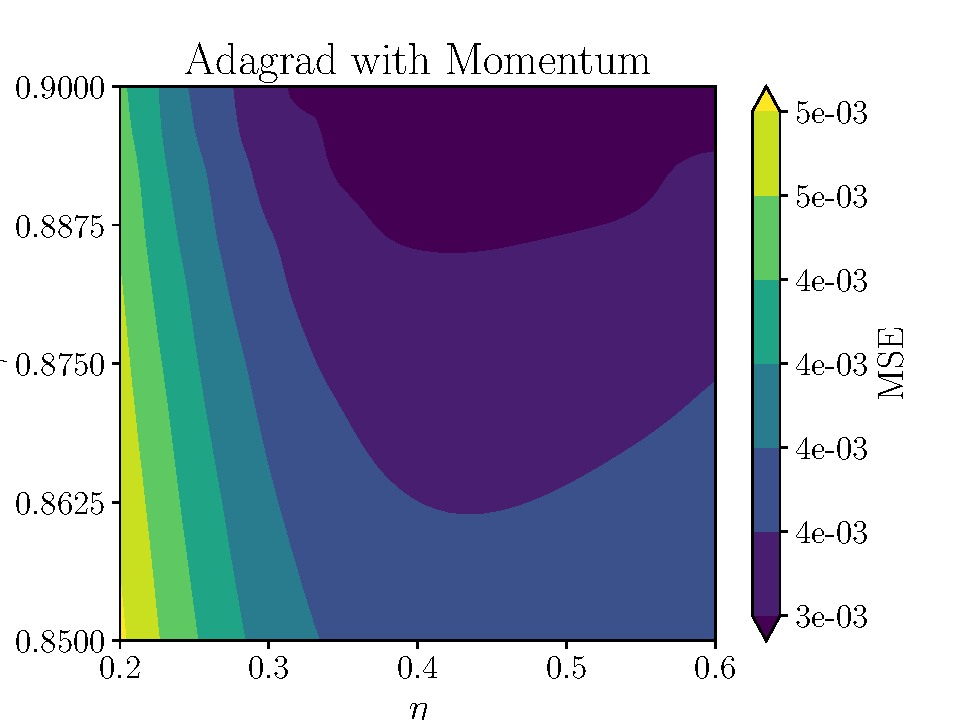
\includegraphics[width = 0.475\textwidth]{../figs/AdagradMomentum_eta_gamma.pdf}
    \caption{Plotting the learning rate against the momentum, using regular AdaGrad}
    \label{fig: AdagradMomentum_eta_gamma}
\end{figure}
\begin{figure}[ht!]
    \centering
    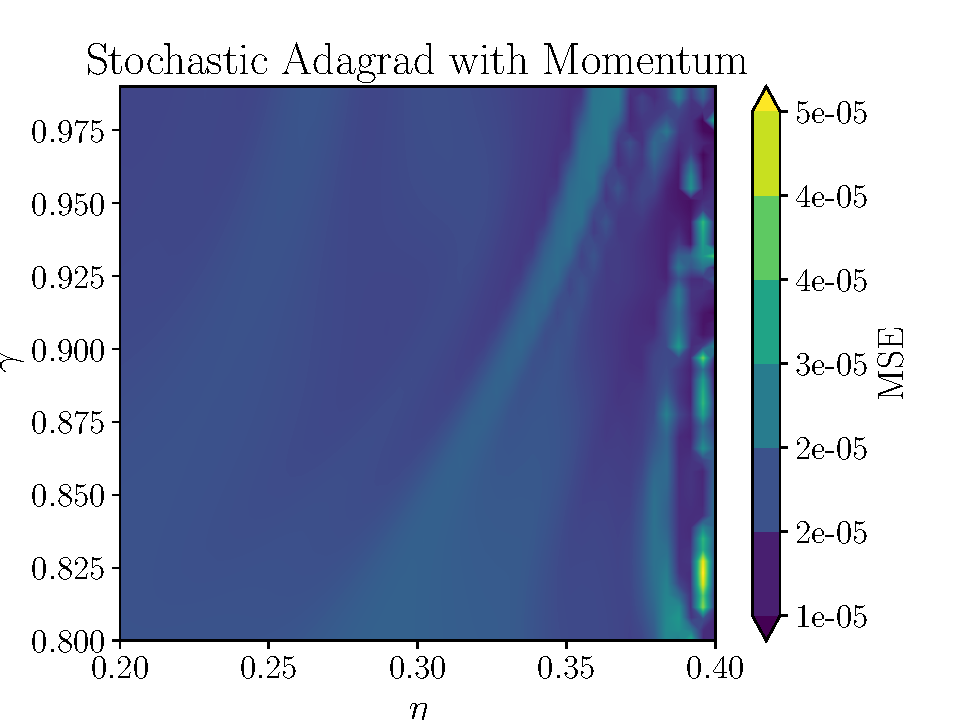
\includegraphics[width = 0.475\textwidth]{../figs/AdagradMomentum_stochastic_eta_gamma.pdf}
    \caption{Plotting the learning rate against the momentum, using stochastic AdaGrad. The batch size is set to 20.}
    \label{fig: AdagradMomentum_stochastic_eta_gamma}
\end{figure}
Exploring further with \cref{fig: AdagradMomentum_eta_gamma} and \cref{fig: AdagradMomentum_stochastic_eta_gamma} we found that the stochastic performed better then plain gradient descent, of 2 orders of magnitude. The stochastic version had an MSE of around \(10^{-5}\), while the plain version had an MSE of around \(10^{-3}\).

\subsubsection{RMSprop}
\begin{figure}[ht!]
    \centering
    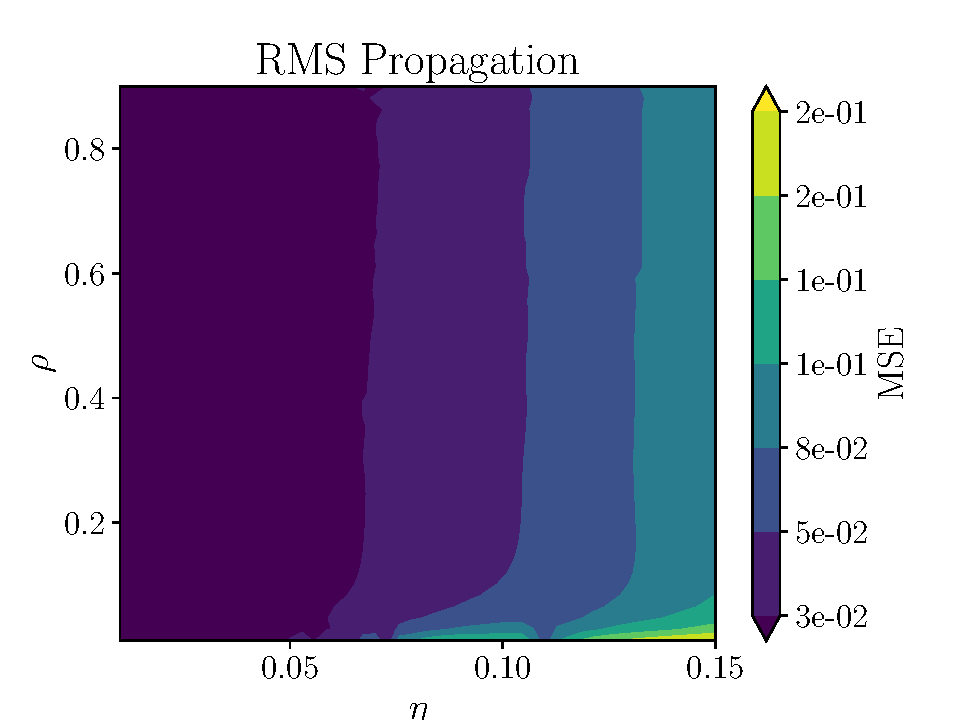
\includegraphics[width = 0.475\textwidth]{../figs/RMS_Prop_eta_rho.pdf}
    \caption{Plotting the learning rate against the decay rate, using RMSprop}
    \label{fig: RMS_Prop_eta_rho}
\end{figure}

\begin{figure}[ht!]
    \centering
    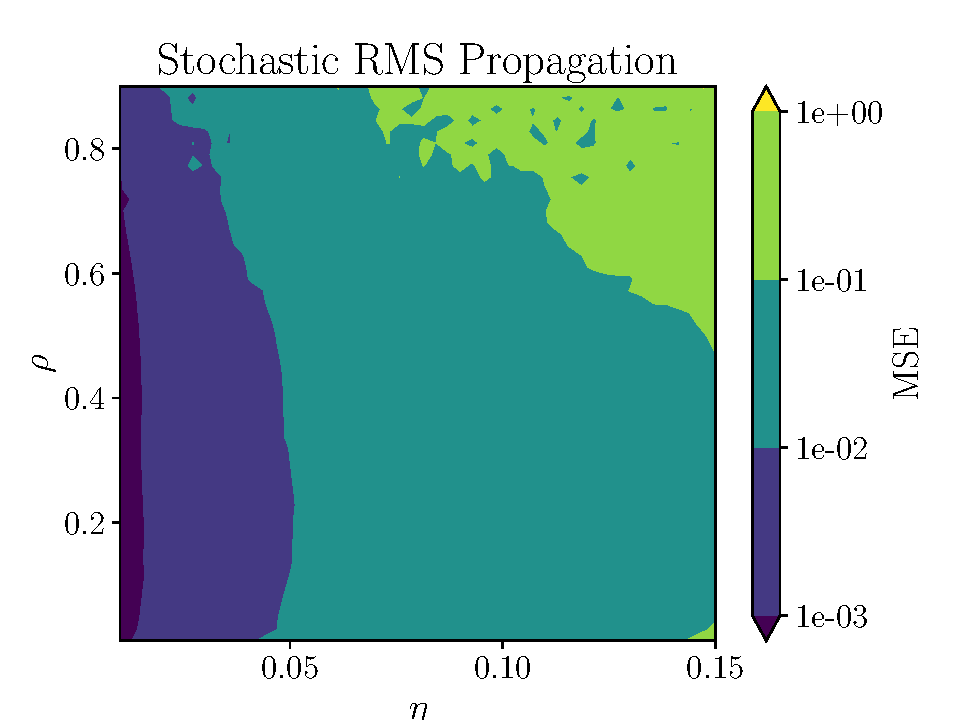
\includegraphics[width = 0.475\textwidth]{../figs/RMS_Prop_stochastic_eta_rho.pdf}
    \caption{Plotting the learning rate against the decay rate, using stochastic RMSprop. The batch size is set to 20.}
    \label{fig: RMS_Prop_stochastic_eta_rho}
\end{figure}
The RMS propagation method was very sensitive to the learning rate. As seen in \cref{fig: RMS_Prop_eta_rho} and \cref{fig: RMS_Prop_stochastic_eta_rho}, there was only a narrow range of learning rates that gave good results. Outside of this range, computation became unstable, and a lot of NaN values were produced. The stochastic version performed better than the plain version, with an MSE of around \(10^{-3}\) compared to \(10^{-2}\). Looking closer at the MSE values of the stochastic variant, we found some spots with MSEs with a value around \( 10^{-4} \). For the plain version, we found some spots with an MSE of around \( 10^{-3} \).

\subsubsection{Adam}
\begin{figure}[ht!]
    \centering
    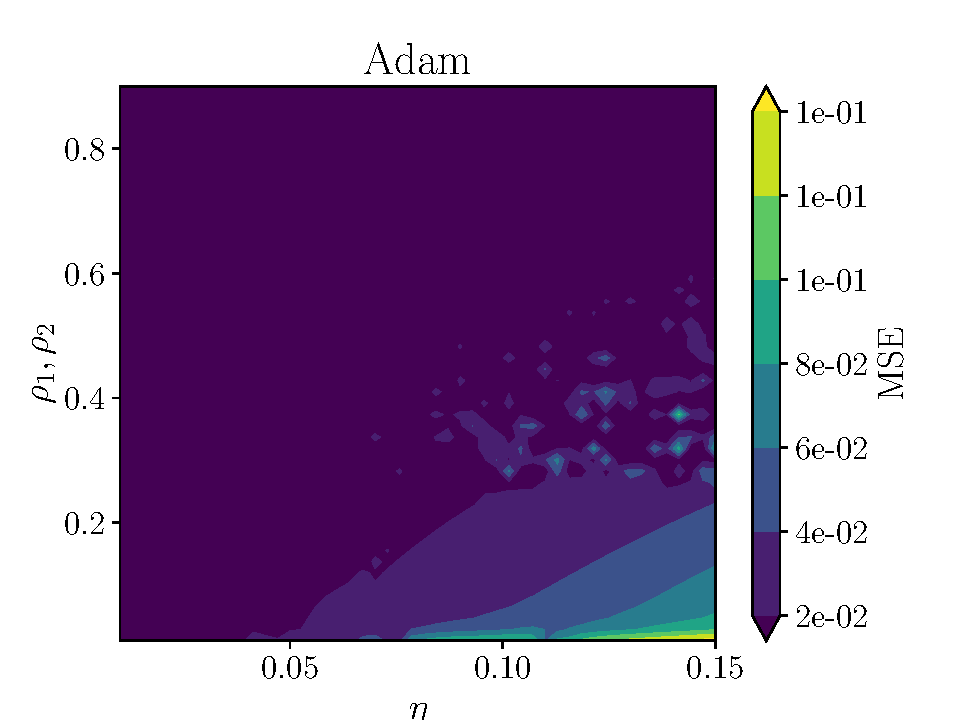
\includegraphics[width = 0.475\textwidth]{../figs/Adam_eta_rho.pdf}
    \caption{Plotting the learning rate against the decay rate. We have set the same value for $\rho_1$ and $\rho_2$, using Adam}
    \label{fig: Adam_eta_rho.pdf}
\end{figure}
\begin{figure}[ht!]
    \centering
    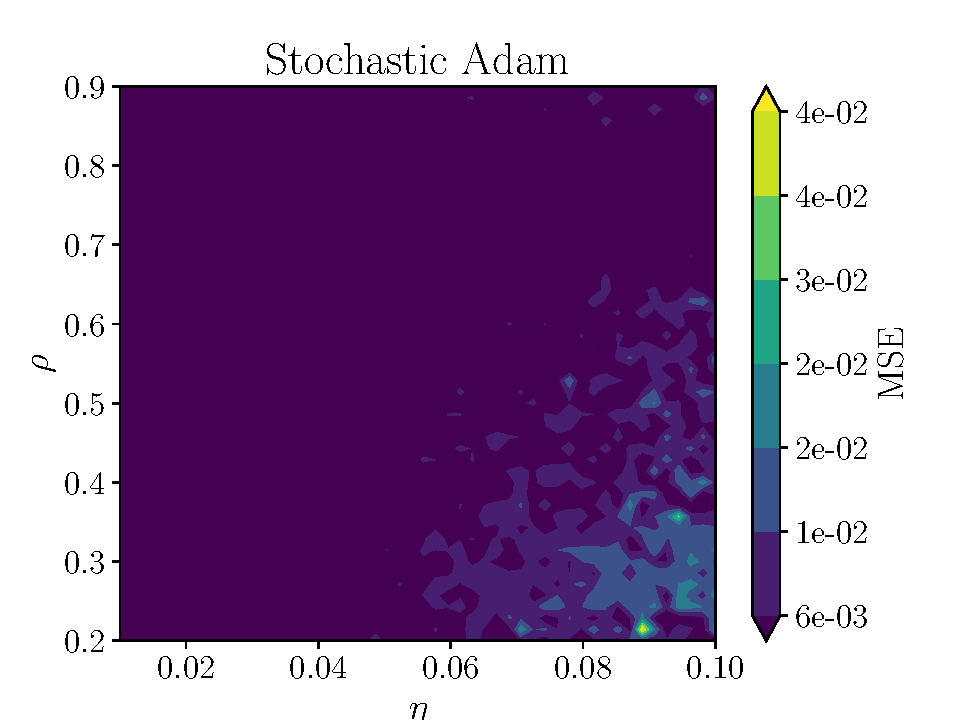
\includegraphics[width = 0.475\textwidth]{../figs/Adam_stochastic_eta_rho.pdf}
    \caption{Plotting the learning rate against the decay rate, using stochastic Adam. The batch size is set to 20, and the same value for $\rho_1$ and $\rho_2$ is used.}
    \label{fig: Adam_stochastic_eta_rho.pdf}
\end{figure}

The Adam optimization method was both unstable and very sensitive to the learning rate. As seen in \cref{fig: Adam_eta_rho.pdf} and \cref{fig: Adam_stochastic_eta_rho.pdf}, the plain version had at best an MSE of around \(10^{-2}\), while the stochastic version had an MSE of around \(10^{-3}\). The stochastic version had some spots with an MSE of around \(10^{-6}\). The plain version had some spots with an MSE of around \(10^{-4}\).

\clearpage

\subsection{Neural Networks Regression}

Our analysis of feed-forward neural networks began with the Franke function regression problem, allowing us to validate our implementation and explore the effects of various hyperparameters. The results demonstrate that our neural network implementation achieves robust performance across a wide range of configurations, with optimal models achieving MSE values around \( 10^{-3} \) and \( R^2 \) scores above 0.95.

\begin{figure}[h!]
    \begin{minipage}{\textwidth}
        \centering
        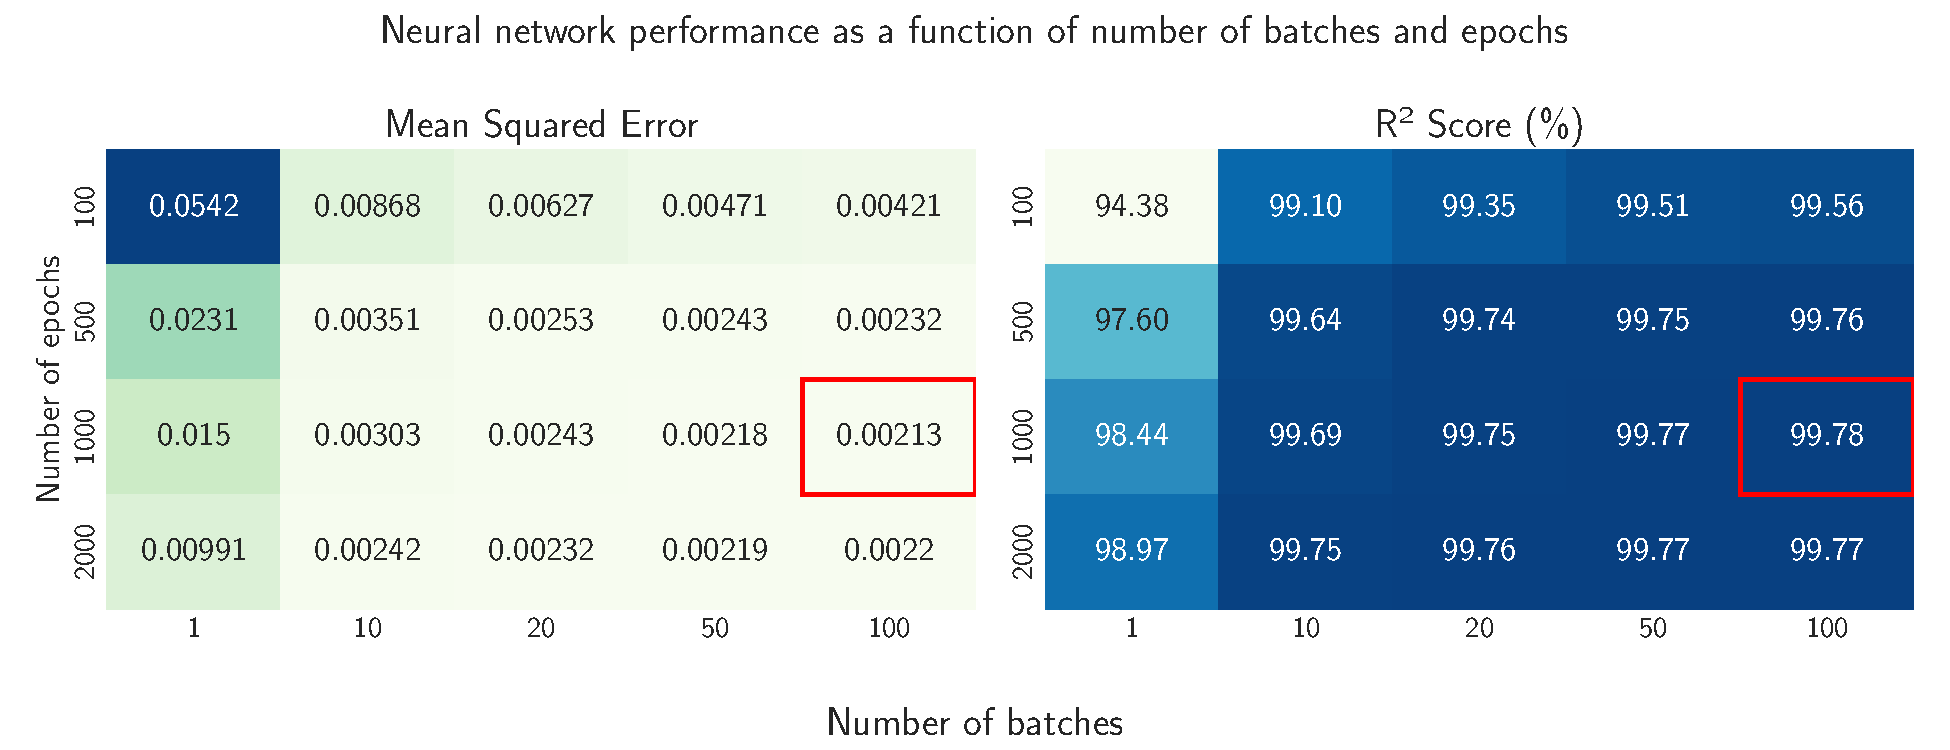
\includegraphics[width = .9\textwidth]{../figs/c_batch_epoch.pdf}
        \caption{The effect of number of epochs and epochs on the Franke function regression problem. The plot shows the MSE and \( R^2 \) scores for different combinations of batches and epochs, with the optimal values highlighted in red.}
        \label{fig:NN_Franke_batch_epoch}
    \end{minipage}
\end{figure}

The clear trend in \cref{fig:NN_Franke_batch_epoch} more batches and epochs lead to better performance, with the optimal model using 1000 epochs and 100 batches. The model shows stable performance across a wide range of batch sizes and epochs, with MSE values around \( 10^{-3} \) and \( R^2 \) scores above 0.95. The improvements in both MSE and $R^2$ show diminishing returns as we increase either epochs or batches.

Moving from 100 to 1000 epochs yields substantial improvements in MSE (reducing it by roughly $60-70\%$ across all batch sizes), but the gains from 1000 to 2000 epochs are much smaller ($10-20\%$ reduction). Similarly, while increasing from 1 to 20 batches significantly improves performance, further increases to 50 or 100 batches yield only marginal benefits. This suggests that a configuration using $20-50$ batches with 1000 epochs represents an efficient compromise between model performance and computational cost

\clearpage

\onecolumngrid
\begin{figure}[h!]
    \begin{minipage}{\textwidth}
        \centering
        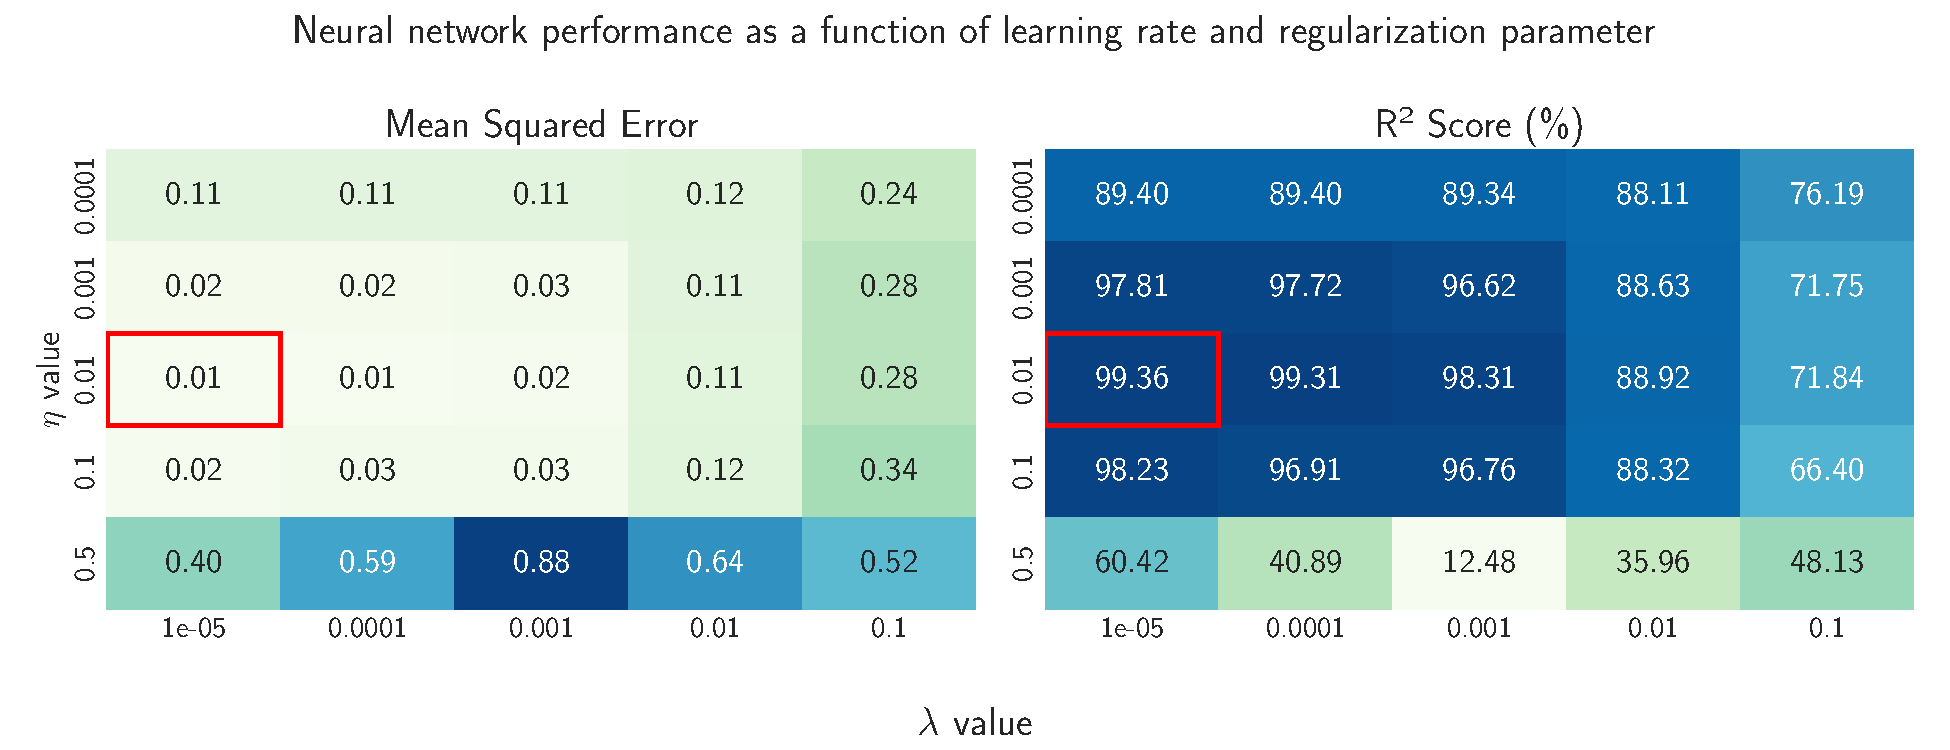
\includegraphics[width = .9\textwidth]{../figs/c_eta_lambda.pdf}
        \caption{The effect of learning rate and regularization strength on the Franke function regression problem. The plot shows the MSE and \( R^2 \) scores for different combinations of learning rate and regularization strength, with the optimal values highlighted in red.}
        \label{fig:NN_Franke_eta_lambda}
    \end{minipage}
\end{figure}
\twocolumngrid

Our feed-forward neural network demonstrated consistently strong performance on the Franke function regression task across a range of hyperparameters. As shown in \cref{fig:NN_Franke_eta_lambda}, the model achieves stable MSE scores around $10^{-3}$ and $R^2$ scores above 0.99 for combinations of learning rates $ \eta $ in the range $ 10^{-1} $ to $ 10^{-3}$ and regularization strengths $ \lambda $ in $ 10^{-3} $ to $ 10^{-5}$ . The model only shows significant performance degradation with the highest tested learning rate ($\eta = 0.5$), suggesting robust behavior across most of the hyperparameter space.

\onecolumngrid
\begin{figure}[h!]
    \begin{minipage}{\textwidth}
        \centering
        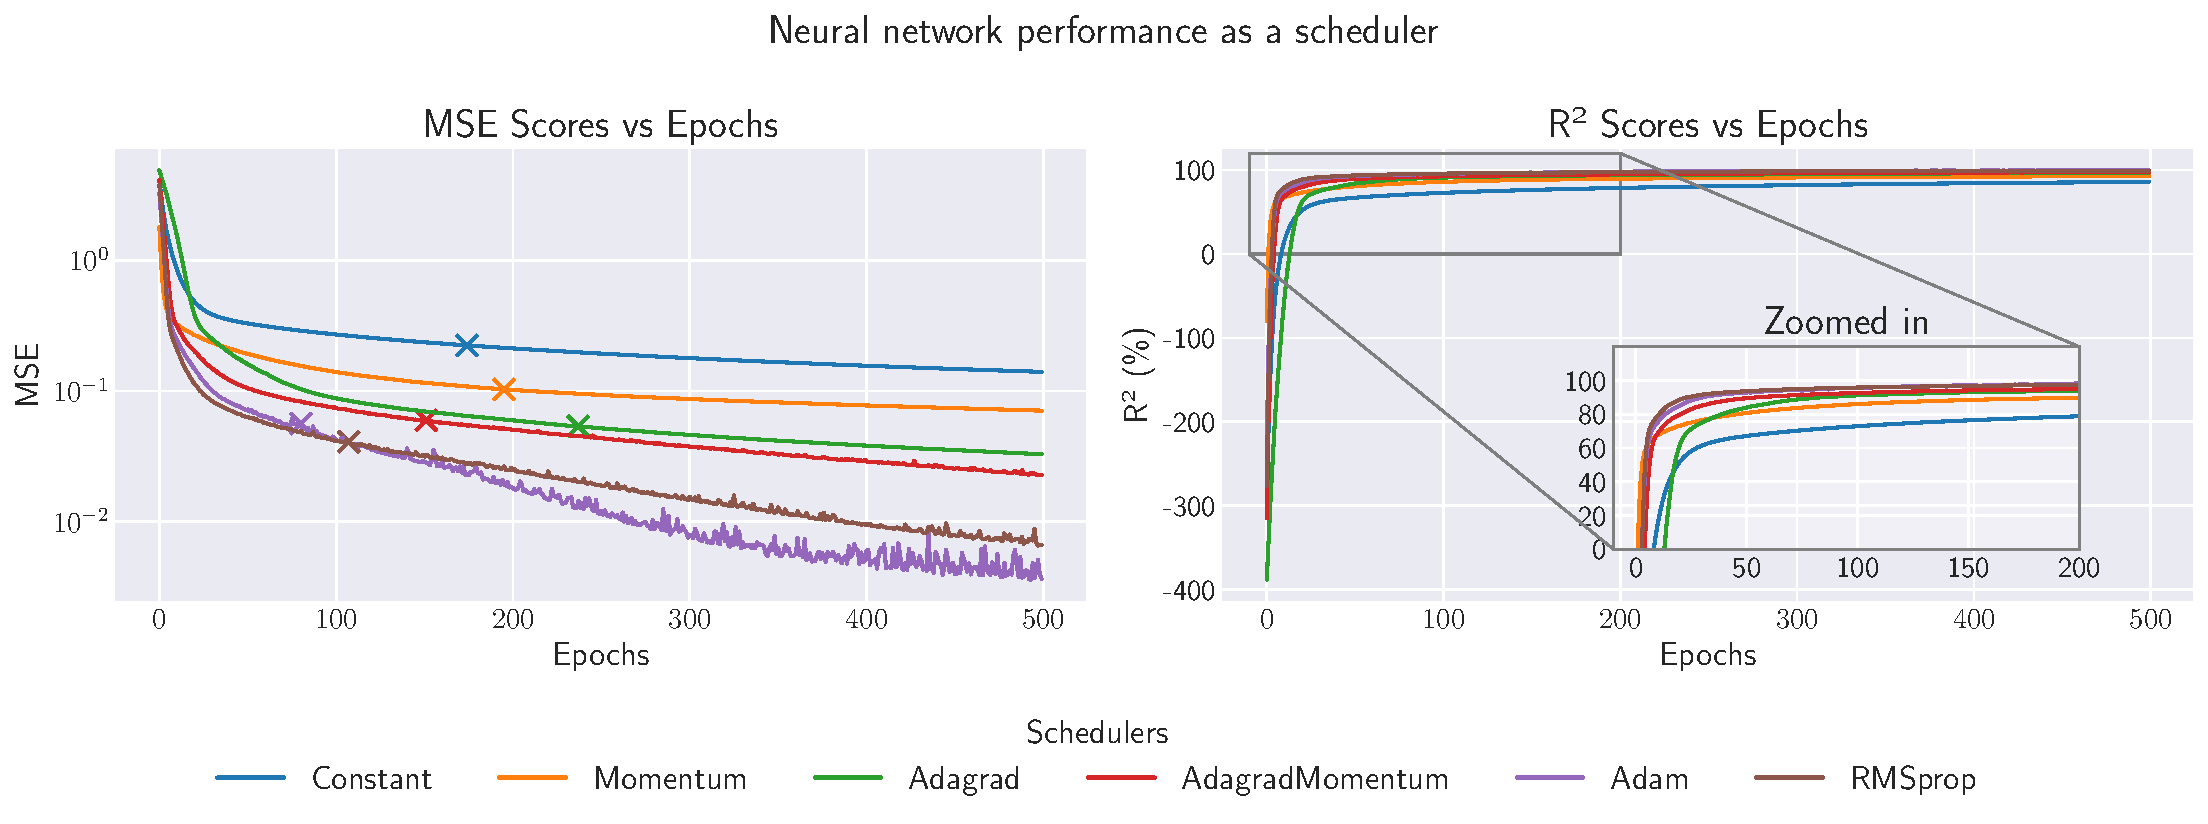
\includegraphics[width = .9\textwidth]{../figs/b_schedulers.pdf}
        \caption{The effect of different learning rate schedulers on the Franke function regression problem. The plot shows the training MSE and \( R^2 \) scores for different learning rate schedulers as a function of epochs. The schedulers MSEs are marked with a cross indicating at which epoch convergence was reached.}
        \label{fig:NN_Franke_schedulers}
    \end{minipage}
\end{figure}
\twocolumngrid

The comparison of different optimization schedulers in \cref{fig:NN_Franke_schedulers} shows that all implemented methods have varying success with plain momentum, both Adagrads and Adam performing the best. The marked convergence points indicate that both Adagrad methods are slightly faster to converge than the other methods. As the criteria for convergence is chosen somewhat arbitrarily, as described in \cref{subsec:nn_schedulers}, the marked crosses may not showcase where the schedulers actually converge, but gives insight into when the learning rates are slowing down relative to each other as the networks are training. The figure also suggest that given enough epochs, both Adagrads, Adam and plain momentum will converge to an mse of just around of \( 10^{-2} \) and an \( R^2 \) score above of 0.95. RMSprop shows the same unstability found in \colorbox{magenta}{REF TO RMSprop} of our gradient descent analysis.

\clearpage

\onecolumngrid
\begin{figure}[h!]
    \begin{minipage}{\textwidth}
        \centering
        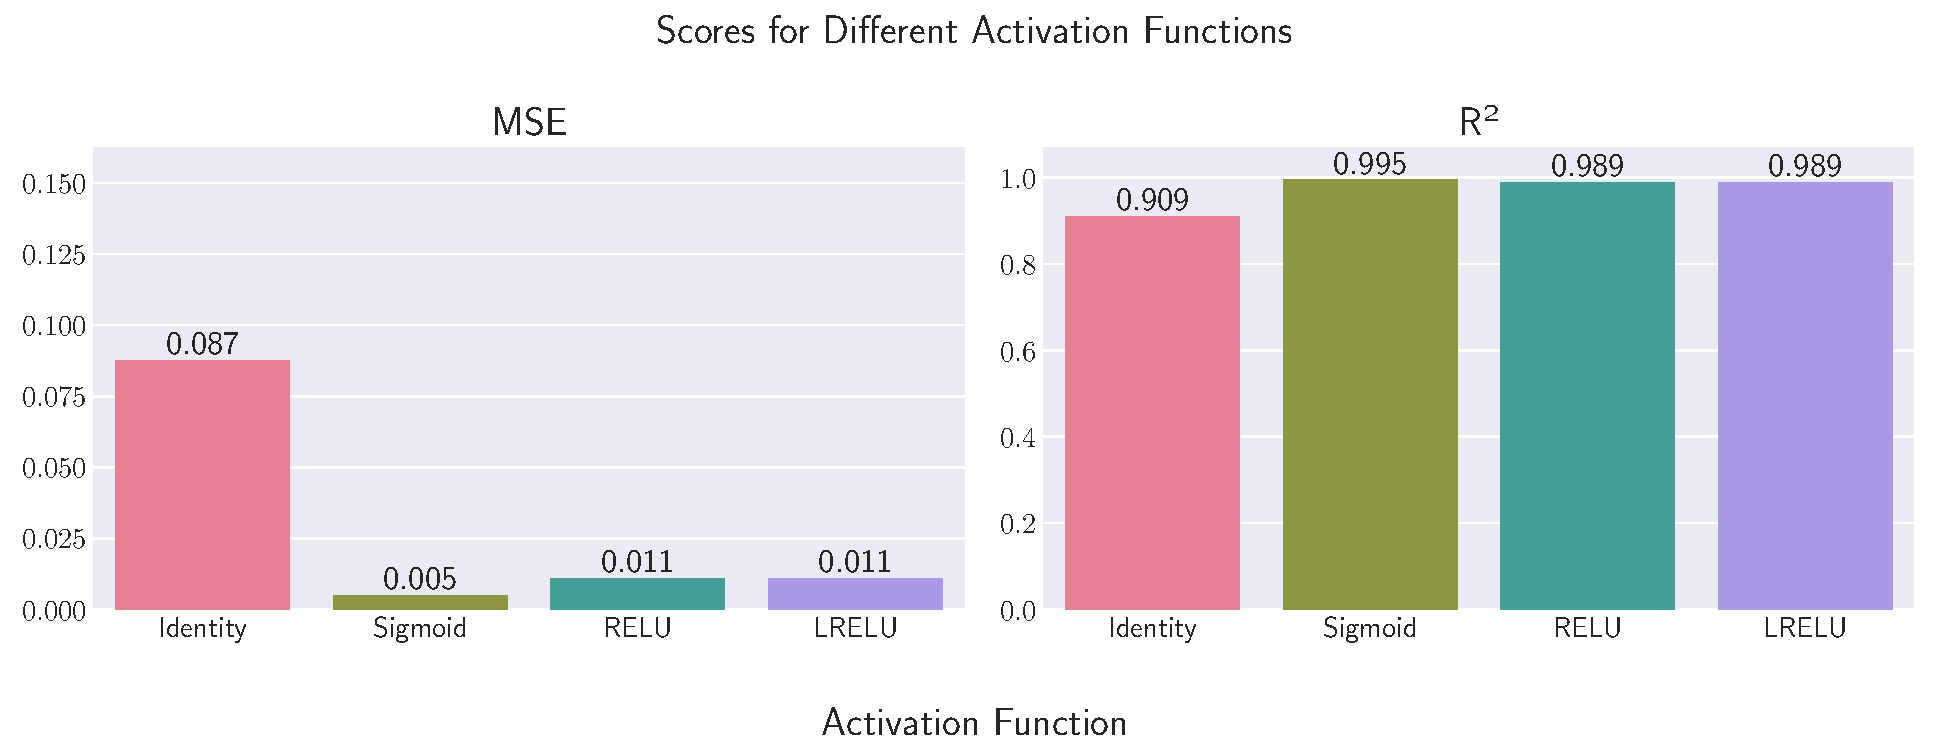
\includegraphics[width = .9\textwidth]{../figs/c_activation_funcs.pdf}
        \caption{The effect of different activation functions on the Franke function regression problem. The plot shows the test MSE and \( R^2 \) scores for different activation functions.}
        \label{fig:NN_Franke_activation}
    \end{minipage}
\end{figure}
\twocolumngrid

Testing different activation functions (\cref{fig:NN_Franke_activation}), reveals similar performance levels among non-linear functions. The sigmoid activation in the hidden layer performs slightly better with an MSE of $0.003$ and $R^2$ of $0.997$, but ReLU and Leaky ReLU follow closely with MSE around $0.010$ and $R^2$ of $0.990$. As expected, removing the non-linear capability of the network by using the identity function in the hidden layer results in significantly worse performance, with an MSE of $\approx0.08$ and $R^2$ of $\approx0.92$.

\onecolumngrid
\begin{figure}[h!]
    \begin{minipage}{\textwidth}
        \centering
        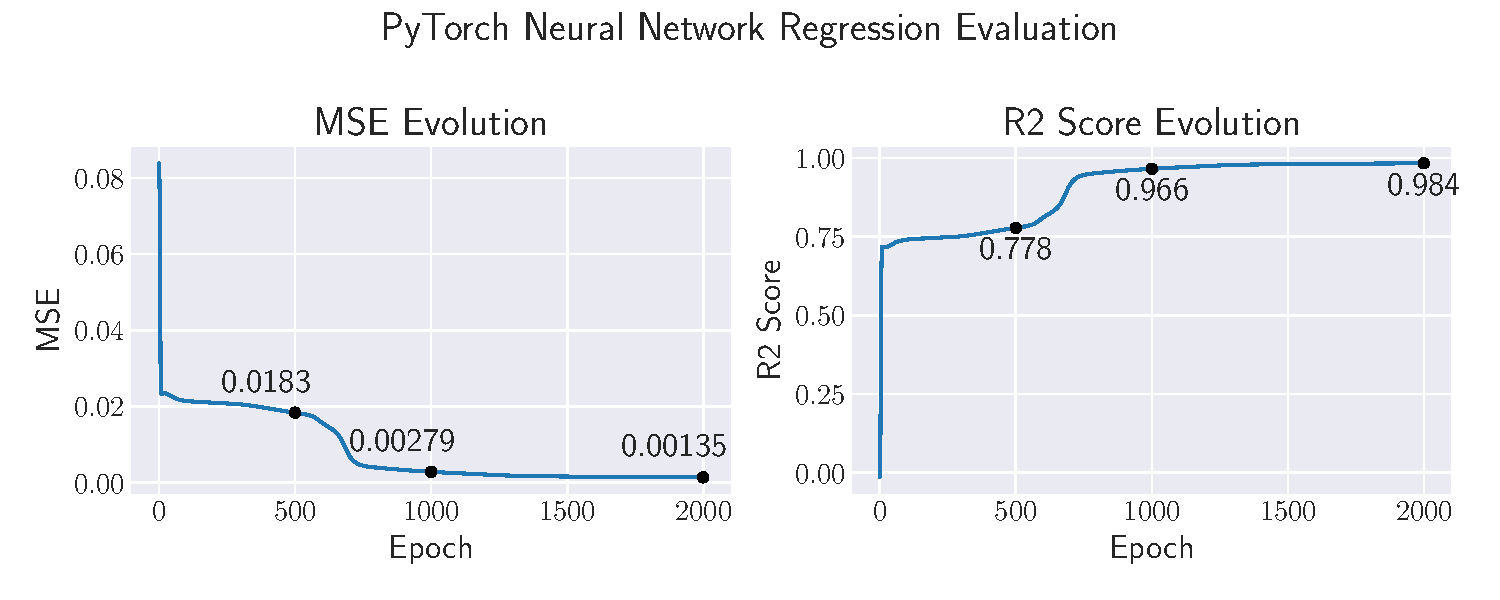
\includegraphics[width = .9\textwidth]{../figs/nn_torch_franke.pdf}
        \caption{PyTorch neural network regression on the Franke function. The plot shows the training and test MSE and \( R^2 \) as a function of epochs. The plots are annotated with the values at epochs 500, 1000 and 2000}
        \label{fig:NN_Torch_scores}
    \end{minipage}
\end{figure}
\twocolumngrid

Comparing our results with the PyTorch implementation in \cref{fig:NN_Torch_scores}, we see that our model performed similarly to the PyTorch model, settling on an MSE around \( 10^{-3} \) and an \( R^2 \) score over 0.98. An interesting feature in the PyTorch implementation's learning curve is the noticeable 'bump' in scoring metrics around epoch 500, followed by recovery and continued improvement. This behavior is characteristic of the model navigating through different local minima in the loss landscape. Rather than indicating instability, such transitions can actually be beneficial, as they suggest the optimizer is able to escape potential local minima in search of better solutions. This dynamic exploration of the parameter space likely contributes to the model's eventual superior performance and supports our earlier observation about its robustness. In contrast, our implementation's faster convergence might indicate it settles more quickly into the first acceptable minimum it finds.

\clearpage

\onecolumngrid
\subsection{Neural Networks Classification}

\begin{figure}[h!]
    \centering
    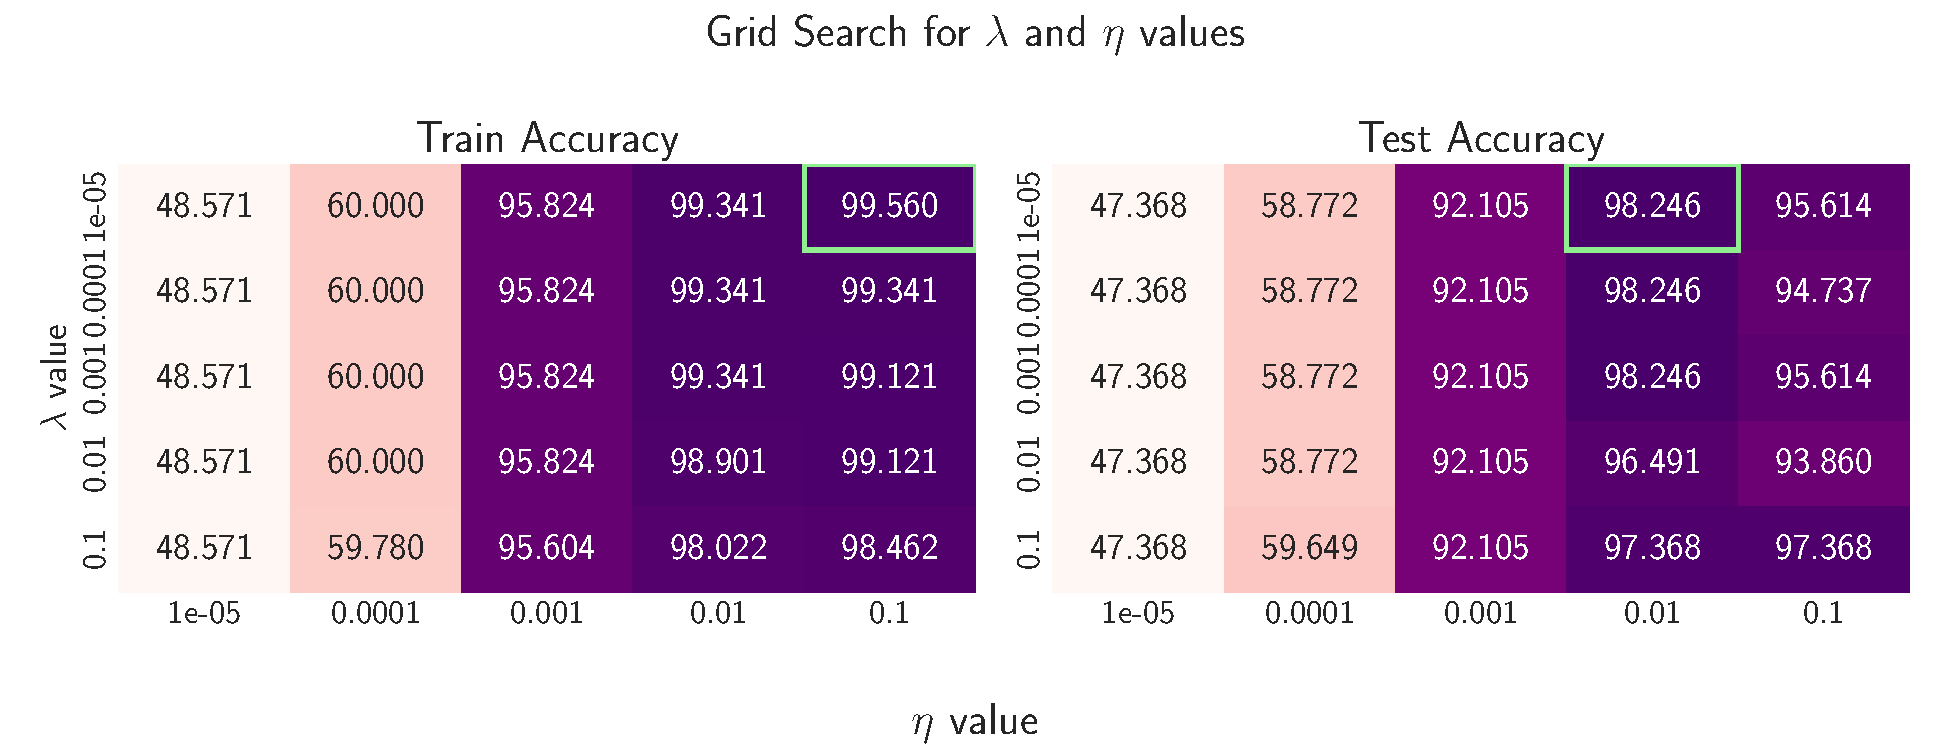
\includegraphics[width = .9\textwidth]{../figs/classification_lambda_eta.pdf}
    \caption{Model performance for different learning rates and regularization strengths on the breast cancer classification problem. The plot shows the training and test accuracy scores for different combinations of learning rate and regularization strength. The optimal values are highlighted in green.}
    \label{fig:NN_Classification_lambda_eta}
\end{figure}
\twocolumngrid

Our feed-forward neural network achieved strong classification performance on the Wisconsin Breast Cancer dataset. As shown in \cref{fig:NN_Classification_lambda_eta}, the model maintains high accuracy($<95\%$) across a broad range of hyperparameter combinations, with optimal performance achieved using learning rates $\eta$ between $10^{-2}$ and $10^{-1}$ and relatively low regularization strengths $\lambda$ . This suggests that for this dataset, the risk of overfitting is relatively low, possibly due to the inherent structure of the feature space that makes the classification boundary relatively clear-cut.

The learning rate appears to be the more critical hyperparameter, with model performance showing high sensitivity to $\eta$ values below $10^{-3}$. This behavior likely stems from the optimizer getting trapped in suboptimal local minima when steps are too small. Conversely, the model's relative insensitivity to regularization strength suggests that the network naturally learns a robust decision boundary without requiring strong parameter constraints.

\onecolumngrid
\begin{figure}[h!]
    \begin{minipage}{\textwidth}
        \centering
        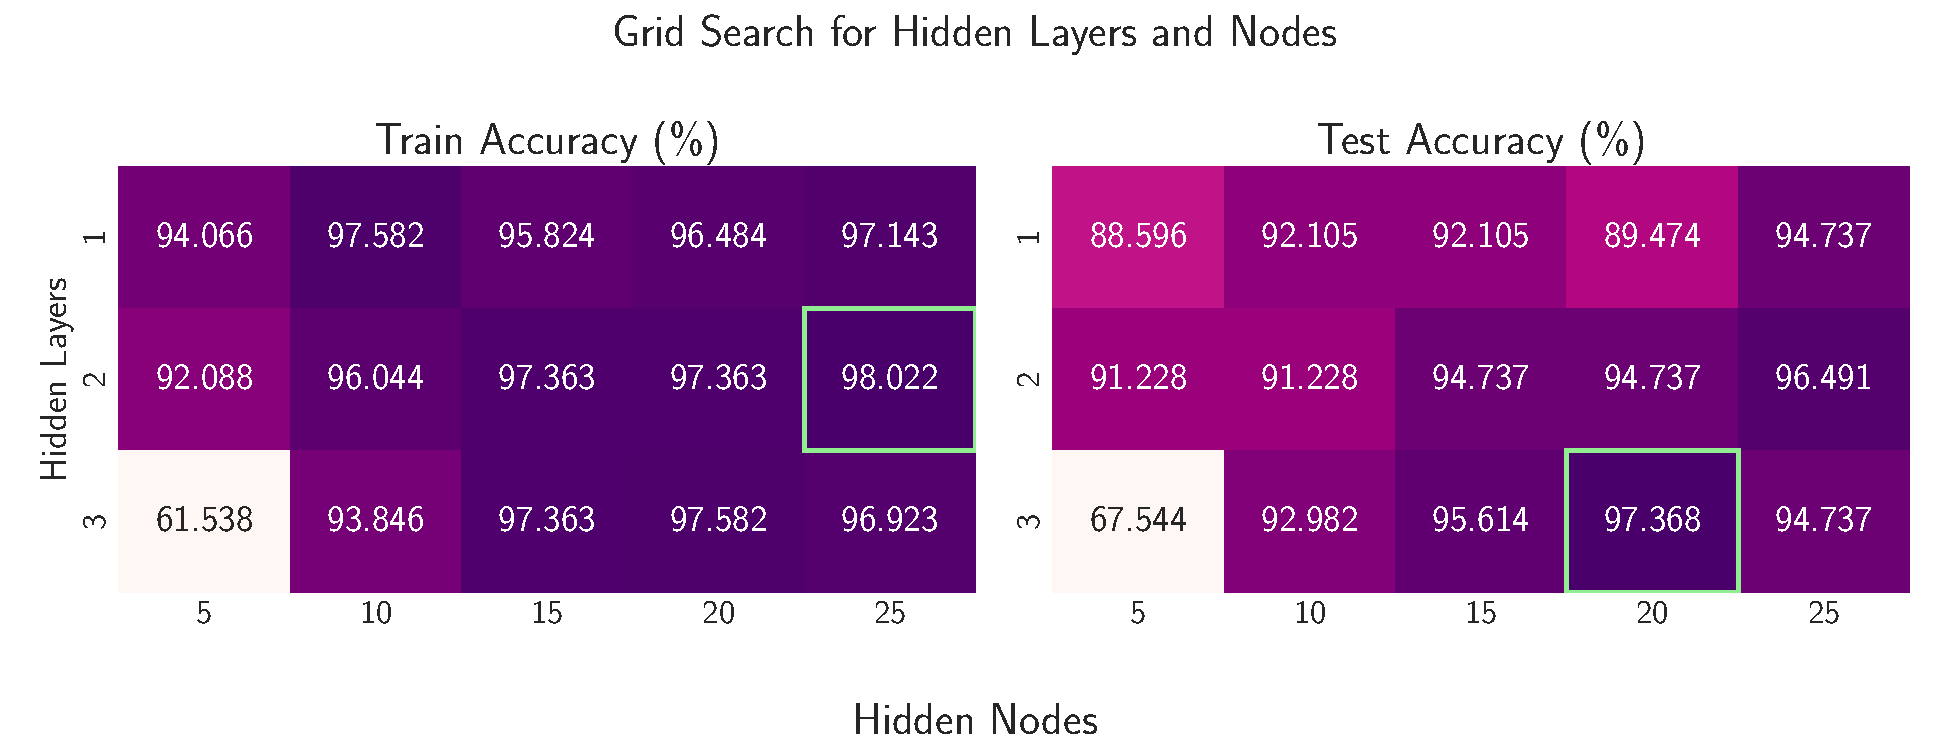
\includegraphics[width = .9\textwidth]{../figs/classification_hidden_layers_nodes.pdf}
        \caption{Model performance for different network architectures on the breast cancer classification problem. The plot shows the training and test accuracy scores for different numbers of hidden layers and nodes. The optimal values are highlighted in green.}
        \label{fig:NN_Classification_hidden_layers_nodes}
    \end{minipage}
\end{figure}
\twocolumngrid

The exploration of network architectures (\cref{fig:NN_Classification_hidden_layers_nodes}) reveals several interesting patterns about model capacity and generalization. Networks with 2-3 hidden layers and 15-25 nodes per layer consistently achieve test accuracies above 96\%, indicating that this level of complexity adequately captures the underlying patterns in the data. However, the degradation in performance with very small networks (5 nodes) is particularly pronounced in deeper architectures, where three-layer networks show training accuracy dropping to 61.5\%. This suggests that while the dataset benefits from some depth in the network, there needs to be sufficient width to create meaningful feature representations at each layer.

The relationship between network depth and model performance provides insights into the dataset's complexity. The fact that accuracy plateaus with modest network sizes suggests that the underlying classification boundary, while nonlinear, does not require extremely complex feature hierarchies to model effectively. This aligns with our understanding of the biological features in the dataset, which are already engineered to be informative for classification.

\clearpage
\onecolumngrid
\begin{figure}[h!]
    \begin{minipage}{\textwidth}
        \centering
        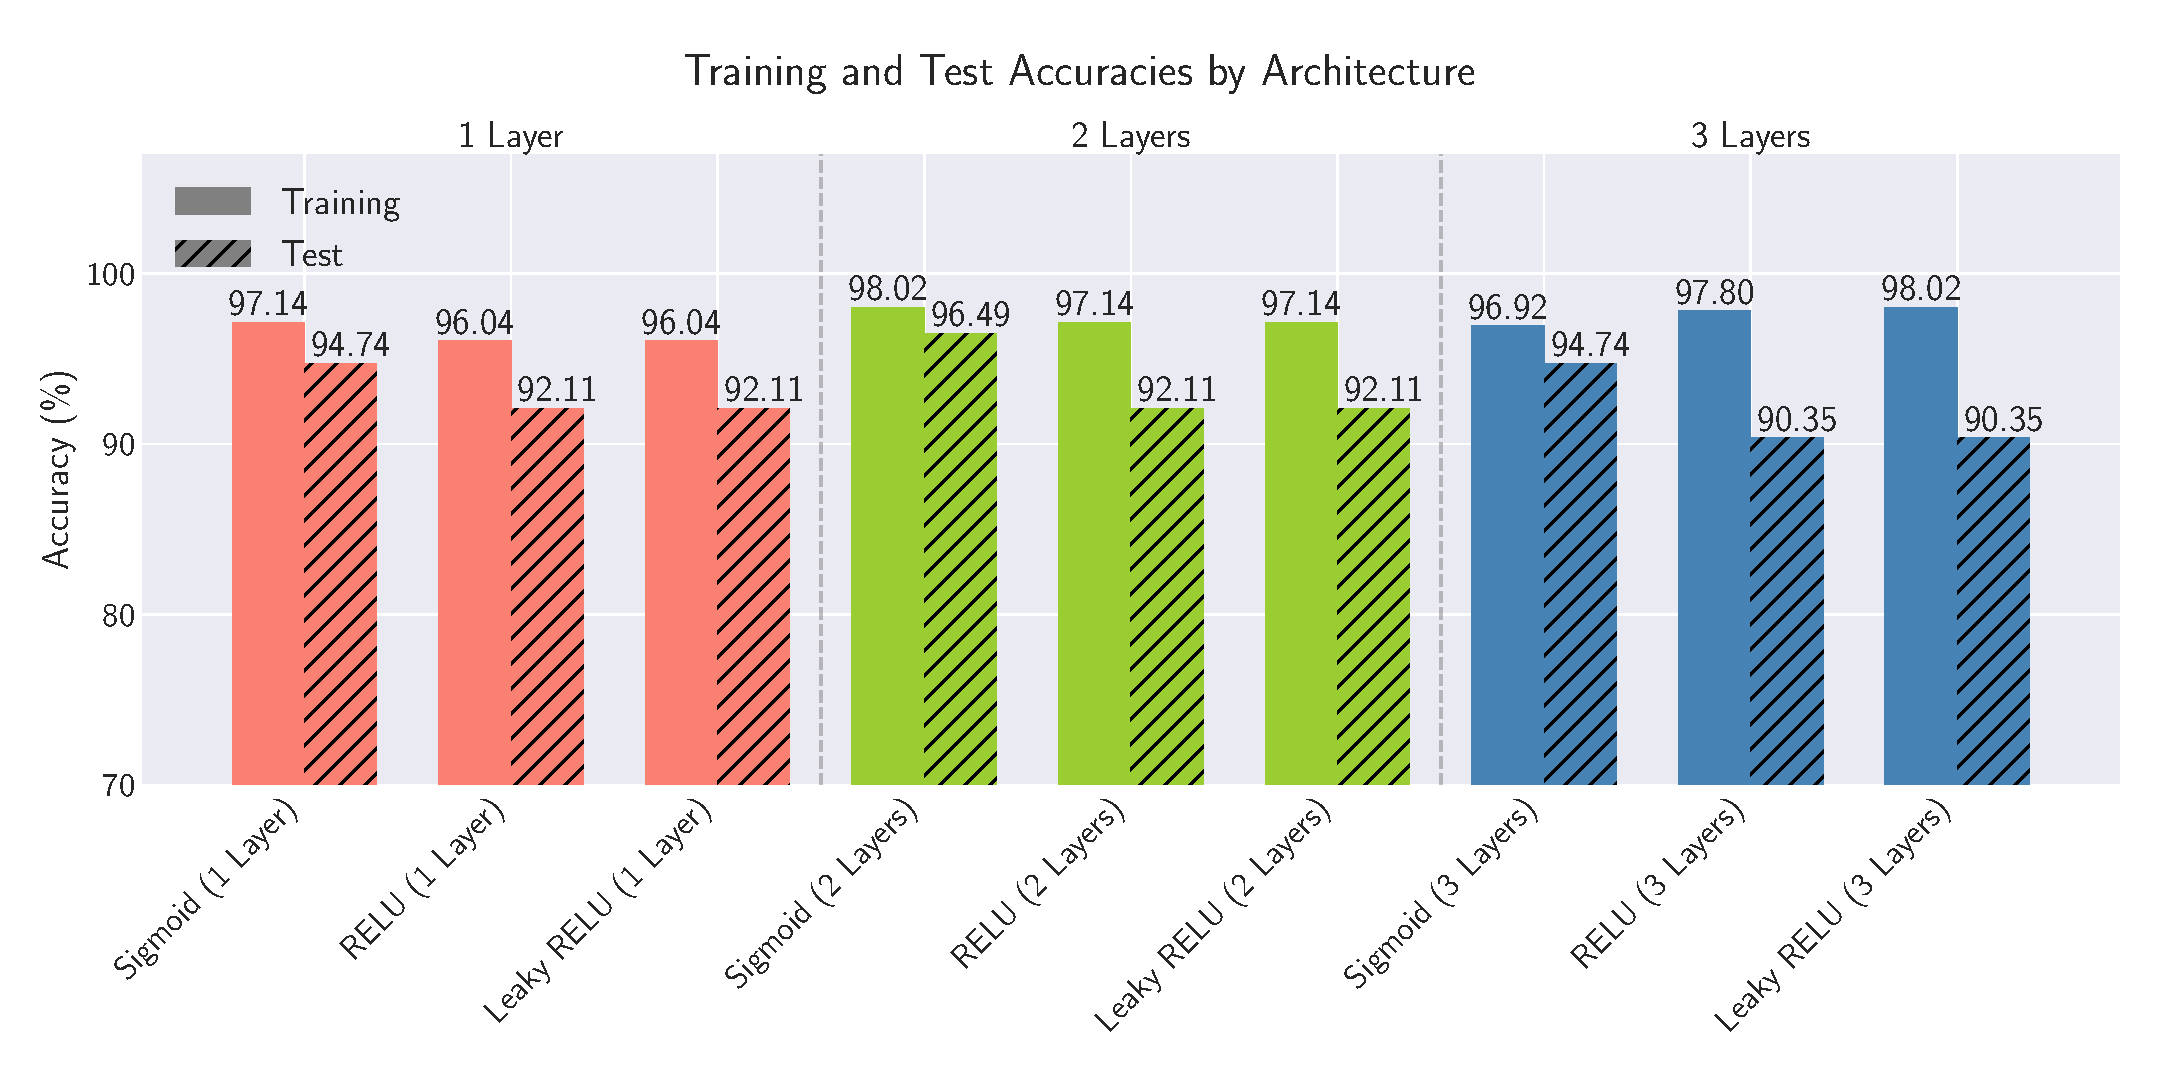
\includegraphics[width = .9\textwidth]{../figs/classification_activations_layers.pdf}
        \caption{Model performance for different activation functions on the breast cancer classification problem. The plot shows the training and test accuracy scores for different activation functions and numbers of hidden layers.}
        \label{fig:NN_Classification_activations_layers}
    \end{minipage}
\end{figure}
\twocolumngrid

Our investigation of activation functions (\cref{fig:NN_Classification_activations_layers}) reveals subtle but important differences in model behavior. While all tested functions perform well, achieving accuracies within 2-3 percentage points of each other, their behavior varies with network depth. Sigmoid activation shows slightly superior performance in single-layer configurations, likely due to its probabilistic interpretation and smooth gradients around the decision boundary. However, ReLU and Leaky ReLU demonstrate better scaling with network depth in training, though this advantage doesn't translate to test performance.

The degradation of test accuracy with increasing network depth, despite improving training accuracy, provides clear evidence of overfitting. This effect is particularly noticeable with ReLU and Leaky ReLU activations in three-layer configurations, where the gap between training and test performance widens significantly. This suggests that while these activations enable faster training and better gradient flow, they may also make the network more prone to memorizing training data when given too much capacity.

\begin{figure}[h!]
    \centering
    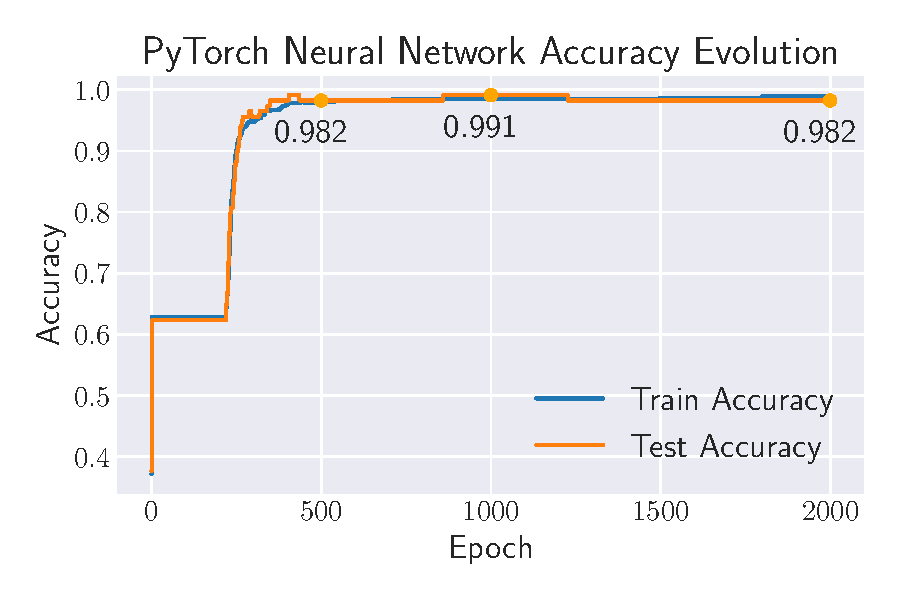
\includegraphics[width =.45\textwidth]{../figs/nn_torch_breast_cancer.pdf}
    \caption{PyTorch neural network classification on the breast cancer dataset. The plot shows the training and test accuracy as a function of epochs. The figure is annotated with the test accuracies at epochs 500, 1000 and 2000.}
    \label{fig:NN_Torch_breast_cancer}
\end{figure}

Comparing our results with PyTorch's implementation (\cref{fig:NN_Torch_breast_cancer}) reveals interesting differences in learning dynamics. The PyTorch model shows more gradual but ultimately more stable learning, achieving consistent test accuracy >98\% after 500 epochs. In contrast, our implementation reaches similar performance levels much faster, as they are alle trained for 20 epochs. This difference likely stems from two factors: first, our simpler implementation may be better suited to this relatively small dataset, avoiding the overhead of PyTorch's more sophisticated optimization techniques. Second, PyTorch's implementation might include additional regularization mechanisms that slow down initial learning but provide better stability.

These results suggest that for datasets of this size and complexity, simpler models with careful hyperparameter tuning can match or exceed the performance of more sophisticated implementations. However, the faster convergence of our model should be interpreted with some caution, as it might indicate a tendency to find good but not optimal solutions quickly, rather than exploring the parameter space more thoroughly as the PyTorch implementation appears to do.

\clearpage
\onecolumngrid
\subsection{Logistic Regression}

\begin{figure}[h!]
    \begin{minipage}{\textwidth}
        \centering
        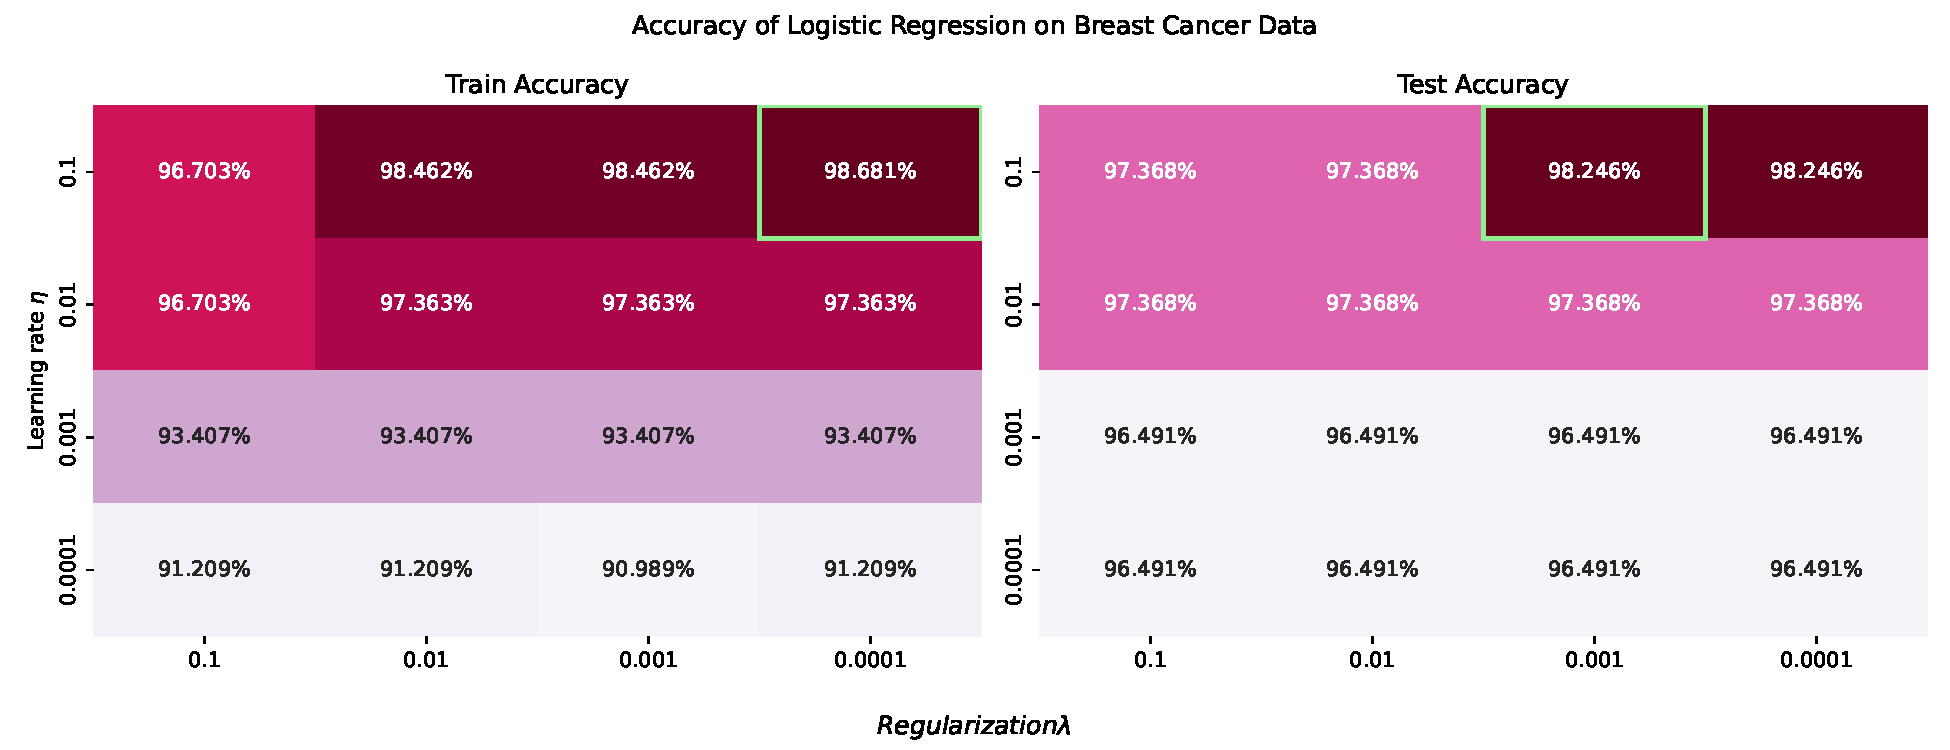
\includegraphics[width = .9\textwidth]{../figs/logistic_regression_gridsearch.pdf}
        \caption{Model performance for different learning rates and regularization strengths on the breast cancer classification problem using logistic regression. The plot shows the training and test accuracy scores for different combinations of learning rate and regularization strength. The optimal values are highlighted in green.}
        \label{fig:logistic_regression_gridsearch}
    \end{minipage}
\end{figure}
\twocolumngrid

Our logistic regression implementation achieves high performance on the breast cancer dataset, with test accuracies consistently above 96\% across most hyperparameter combinations. \cref{fig:logistic_regression_gridsearch} shows that performance is robust across a wide range of learning rates and regularization strengths, with optimal test accuracy of 98.2\% achieved at $\eta$ = 0.0001 and a regularization strength of 0.1. The model demonstrates good generalization, with test accuracies closely matching training accuracies across the parameter space.

\begin{figure}[h!]
    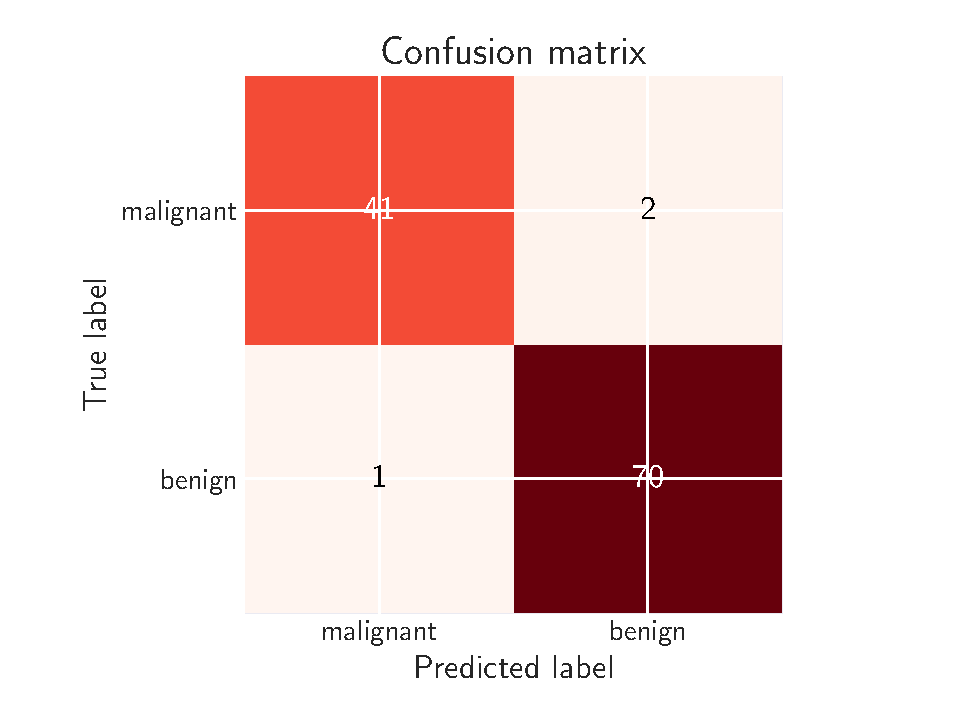
\includegraphics[width =.45\textwidth]{../figs/confusion_matrix.pdf}
    \caption{Confusion matrix for the breast cancer classification problem with Skikit's Logistic Regression. The plot shows the confusion matrix for the test set, with the number of true positives, true negatives, false positives, and false negatives.}
    \label{fig:confusion_matrix}
\end{figure}

The confusion matrix from scikit-learn's implementation (\cref{fig:confusion_matrix}) shows excellent classification performance with only 3 misclassified samples out of 114 test cases. The model correctly identified 41 out of 43 malignant cases and 70 out of 71 benign cases, demonstrating balanced performance across both classes. The similar performance between our implementation and scikit-learn's validates our approach while suggesting that the classification task may be well-suited for linear decision boundaries.

% \vspace*{-2.5pt}
